

% \begin{figure*}[p]
% \fbox{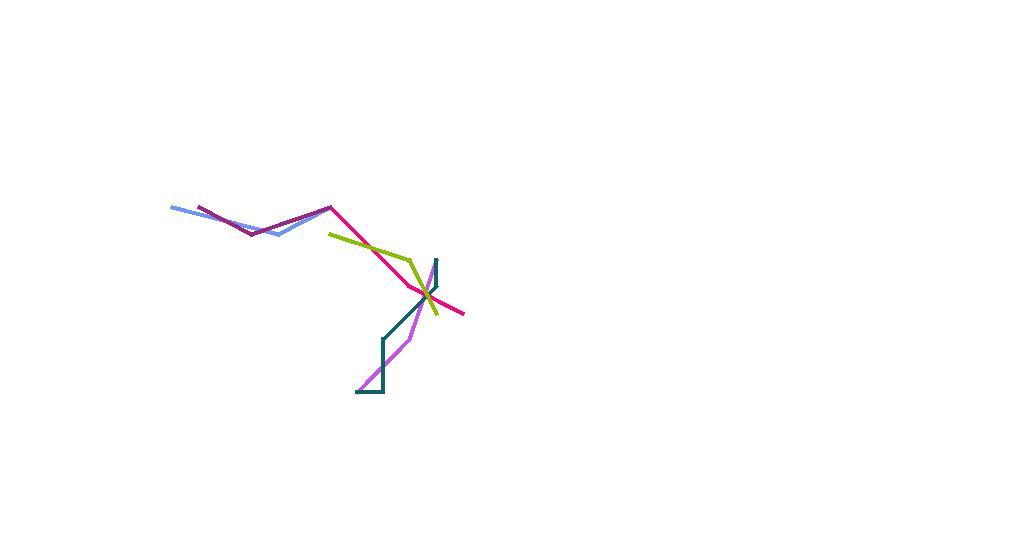
\includegraphics[width=0.85\linewidth]{1-6.png}}
% \end{figure*}
% 
% 
% \begin{figure*}[p]
% \fbox{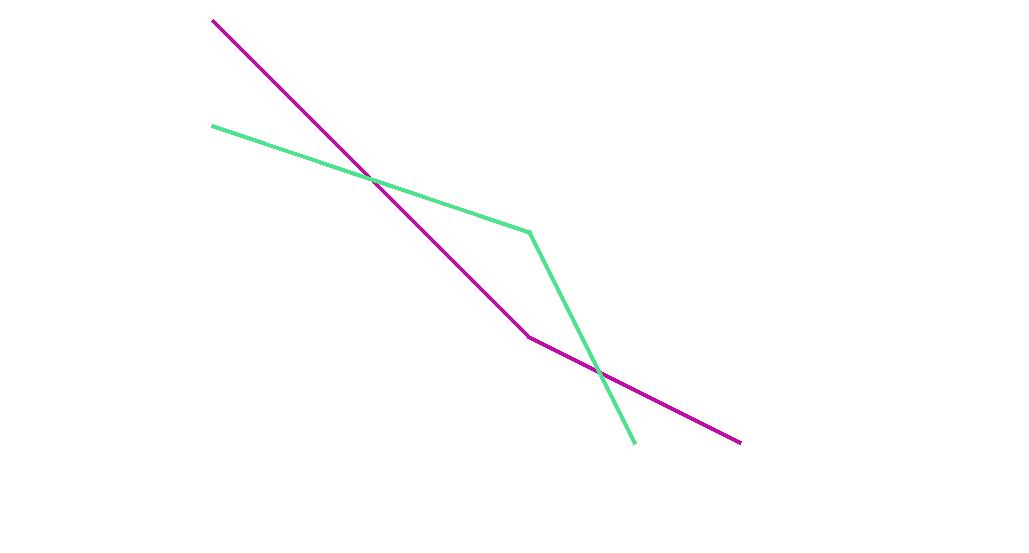
\includegraphics[width=0.65\linewidth]{3-4.png}}
% \end{figure*}
% 


% \section{User-interfaces}
% 
% 
% 
% 
% \framebox[4in][l]{\prompt \cmd{this is a command, short}}


% 
\index{test0.dat}



\vspace{-7\baselineskip}\footnotetext{You must download the program and the example data set, please see page \pageref{download}.}
\vspace{7\baselineskip}




First of all, we must open the program (see page \pageref{openprogram}), read the data set and define the values of the parameters, to be used in this analysis. For test0.dat we will use the following values:

\begin{center}
\begin{tabular}{ll}
\tui{c}ut & 0.25\\
\tui{r}ules & 0.75 0.5 1\\
\tui{m}inimal congruence & 0.8
\end{tabular}
\end{center}


\vspace{-7\baselineskip}\footnotetext{please remember:\\
to set each of these parameters you have to type the letters inside the square brackets [ ] and write the corresponding value followed by and [enter] or [return]}
\vspace{7\baselineskip}


\textbf{Search options}: Once the parameters have been defined, we will search for the general patterns of distribution. 

As we might have similar initial MSTs, we need to reduce them taking into account the similarity among the individual tracks to join
(gro\tui{u}p of tracks) and the value of \tui{m}inimal congruence fixed.
 
In the case of test0.dat, we gro\tui{u}p from the track number 1 [first] to the track number 6 [last]. Thus, we find whether there are similar individual tracks that can be consider as the same track, and those tracks will be joint. 


Later, we might need to redefine the values of the paramaters, in the case of test0.dat we will set:
\index{parameters:modify}


\begin{center}
\begin{tabular}{ll}
\tui{c}ut & 0.5\\
\tui{r}ules & 1.5 1 2\\
\tui{m}inimal congruence & 0.8
\end{tabular}
\end{center}



Then, Typing \tui{a}ll, we will find the congruent segments for each individual tracks in order to delimitate the generalized tracks or distributional patterns of species.

Finally, we need to eliminate those redundant generalized tracks, typing again \tui{u}, but joint from the track number 7  to the track 9, because first six tracks are individual tracks.

\textbf{Write a kml file}

Now, we need to write our results (the generalized tracks) in a kml file. To do that, first we must type \tui{k} and \tui{+} to activate the output to the  kml file. The kml info must change from FALSE to TRUE. Then, we will use \tui{w} if we want to write the whole information of the analysis including: individual tracks, and generalized tracks, or we can type \tui{e} to write only the generalized tracks into the kml file.
\vspace{-7\baselineskip}\footnotetext{.kml file extension is mandatory with googleearth, otherwise googleearth will complain and will not open the file}
\vspace{7\baselineskip}

\subsection{Command line interface}
\index{cli:command line interface}

For the command-line user interface we need to specified: 

the input file, 

the output file, 

and the parameters file.


For linux 64 bits:
\vspace{-7\baselineskip}\footnotetext{
CL typography: commands will be  \pname{croizat0}, to indicate that the instruction is named Croizat0 and you must type \pname{croizat0} in your parameter file, the command could be written using lower or upper case.}
\vspace{7\baselineskip}


\framebox[4.3in][l] {\prompt \cmd{ ./{\mt}-64 <input file> <output file> <parameters file>}}


%
%For linux 32 bits:
%
%\framebox[4.4in][l] {\prompt \cmd{ ./{\mt}-32 <input file> <output file> <parameters file>}}
%


For Windows 64 bits:

\framebox[4.4in][l] {\prompt \cmd{ {\mt}-64.exe <input file> <output file> <parameters file>}}


For Windows 64 bits:

\framebox[4.4in][l] {\prompt \cmd{ {\mt}-32.exe <input file> <output file> <parameters file>}}


\textbf{Output file:} it must have an extension .kml. 


\textbf{parameters file:} This interface was designed for parameters/searching strategies defined previously. These search strategies have to be set in the parameters file. There are two main predefined strategies, \pname{croizat0}, and \pname{croizat1}.




The framework of \pname{croizat0} is: 
\begin{enumerate}
 \item Find similar individual tracks [=\tui{u}] from the first, to the last individual track
 \item Calculate the congruent segments among individual tracks (delimitate generalized tracks) [= \tui{a}]
 \item Find similar generalized tracks  [=\tui{u}] from the first, to the last generalized tracks
\end{enumerate}
Therefore, our analysis made with the TUI is a \pname{croizat0} analysis.


The framework of \pname{croizat1} is: 
\begin{enumerate}
 \item Calculate the congruent segments among individual tracks (delimitate generalized tracks) by \tui{a}
 \item Find similar generalized tracks by \tui{u} from the first, to the last generalized tracks
\end{enumerate}

Thus, the commands for the analysis of test0.dat, using par1-search1.txt are:
\index{test0.dat: command line run}

For linux 64 bits:

\framebox[4.4in][l] {\prompt \cmd{ ./{\mt}-64 test0.dat test0.kml par1-search1.txt}}

% 
% For linux 32 bits:
% 
% \framebox[4.4in][l] {\prompt \cmd{ ./{\mt}-32 test0.dat test0.kml par1-search1.txt}}


For Windows 64 bits:

\framebox[4.5in][l] {\prompt \cmd{ {\mt}-64.exe test0.dat test0.kml par1-search1.txt}}

 
 For Windows 32 bits:
 
\framebox[4.5in][l] {\prompt \cmd{ {\mt}-32.exe test0.dat test0.kml par1-search1.txt}}
 


\subsection{Results of test0.dat analysis}


\begin{figure}[!ht]
\begin{center}
 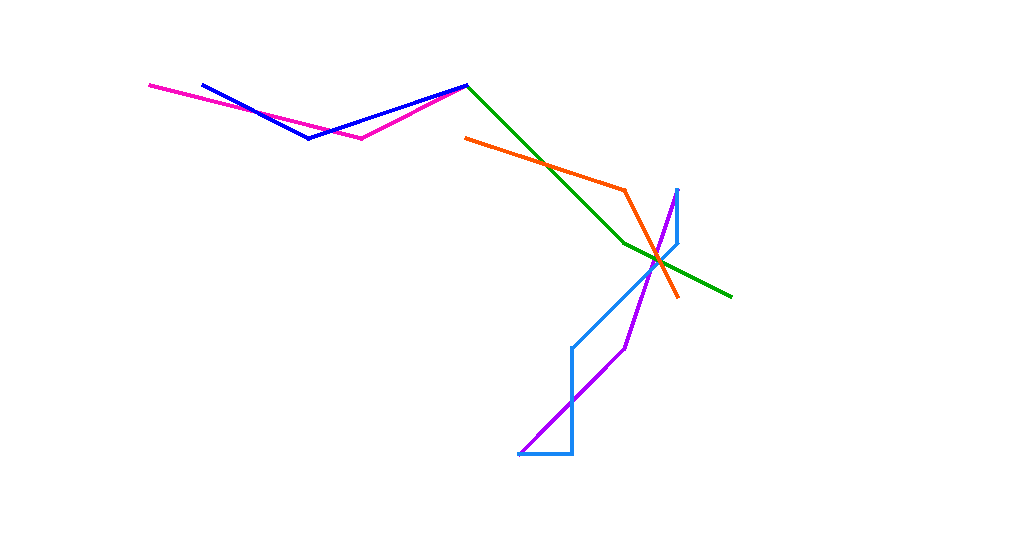
\includegraphics[scale=0.5]{./graphics/mst.png}
 % mst.png: 1029x553 pixel, 96dpi, 27.22x14.63 cm, bb=0 0 772 415
\end{center}
\caption{{\bf Individual tracks from test0.dat}}
\label{Figure1}
\end{figure}


\begin{figure}[!ht]
\begin{center}
 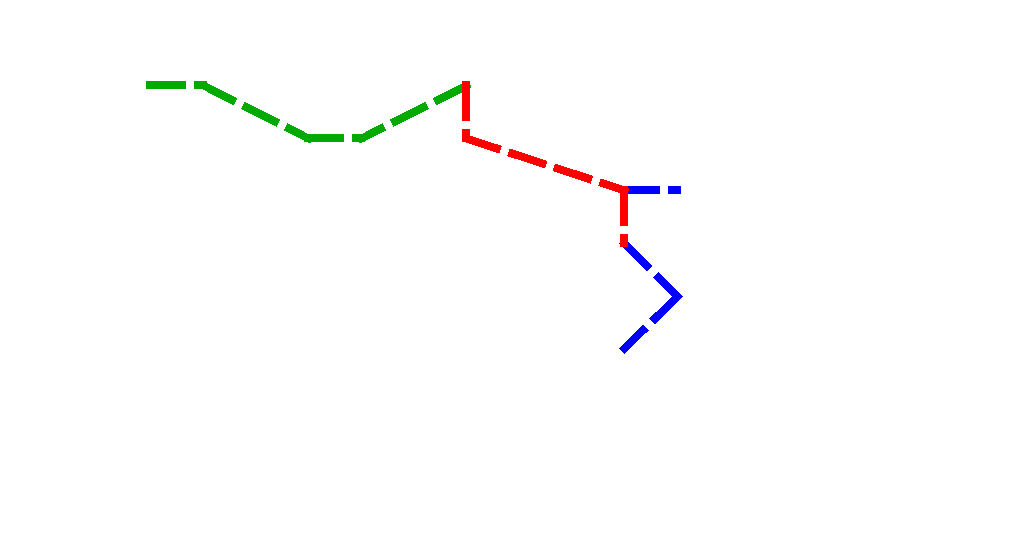
\includegraphics[scale=0.5]{./graphics/gtrack.png}
 % gtrack.png: 1029x553 pixel, 96dpi, 27.22x14.63 cm, bb=0 0 772 415
\end{center}
\caption{{\bf Generalized tracks from test0.dat}}
\label{Figure2}
\end{figure}

